%\documentclass{article}
%\usepackage{graphicx,subfigure}
%\begin{document}

\begin{figure}[!h]
  \centering
  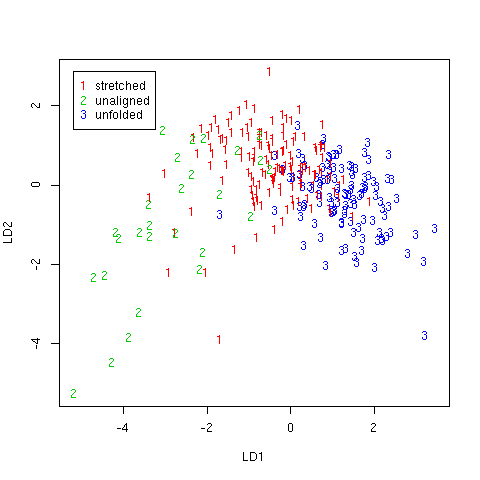
\includegraphics[width=1.1\textwidth]{figplotlda14.png}
  \caption{Plot of the two discriminant function values for the case with all 10  on-sheep traits plus density, IntGpDens, FollperGp, and FollGpArea, showing how the CrimpType groups separate}
  \label{fig:plotlda14}
\end{figure}

%\end{document}

